% 学術論文版（格式版）：SF 考証の内容を除き、品評を受けて主張の射程を調整した版
% 元の版は letter.tex。ビルド: report/letter/ で latexmk -lualatex letter_formal.tex
\documentclass[paper=a4paper,fontsize=10pt,twocolumn,column_gap=2zw,line_length=24zw,number_of_lines=46,head_space=20mm]{jlreq}
\usepackage{amsmath,amssymb,bm}
\usepackage{graphicx,xcolor}
\usepackage{booktabs,array,multirow}
\usepackage{tikz}
\usetikzlibrary{arrows.meta,positioning}
\usepackage[hidelinks]{hyperref}
\usepackage{url}
\graphicspath{{./}{../../figures/}}
\newcommand{\repo}{https://github.com/okamasaya/simulation_AMBAC}
\setlength{\textfloatsep}{8pt plus 2pt minus 2pt}
\setlength{\floatsep}{6pt plus 2pt minus 2pt}
\setlength{\abovecaptionskip}{3pt}
\renewcommand{\arraystretch}{1.08}

\title{\textbf{安価なシミュレーションと校正値は\\フィジカル AI の何を助けるか}\\[0.3em]
\large --- 手足による姿勢制御（AMBAC）を「答えの分かっている試験台」として ---}
\author{simulation\_AMBAC プロジェクト}
\date{2026 年 11 月}

\begin{document}
\twocolumn[
\begin{@twocolumnfalse}
\maketitle
\vspace{-1.5em}
\begin{center}\begin{minipage}{0.9\textwidth}\small
\textbf{概要}\quad
フィジカル AI（身体を持って実世界で動く AI）の開発は、高価な実機、sim-to-real ギャップ、構造のない探索の難しさ、実機の校正という課題を抱える。
本稿は、実機も GPU を前提とする高精細なシミュレータも使えない条件で、CPU だけで動く安価なシミュレーションがこれらの課題のどこまでに答えられるかを、
手足の運動の反作用で胴体の向きを変える AMBAC（Active Mass Balance Auto Control）を試験台として検討する。
AMBAC は基本式が 1 本で、最適解と理論上界が分かる非ホロノミック系であり、学習・制御・校正の手法を「答え合わせ」できる。
(1) 構造を持たない方策は、ループ運動の効果が振幅の 2 次であるために探索に失敗するが、振動子の構造を与えると理論上界の 98\% に達し、人手で設計した制御を上回った。
(2) モデル誤差と外乱の下では、ドメインランダム化で学習した方策の終端誤差は 0.09°で、開ループの最適制御（30.5°）より頑健だった。一方、推進剤の節約は最適制御が担うべき「最初の判断」に集中していた。
(3) 答えを隠した仮想の実機で、姿勢の波形から質量・慣性を推定し、誤差を統計・計算・系統に分けて評価した。微分を使わない推定は、偏りが統計的に有意でなく（50 回の平均で 0.2\% 以下）、1 試行のばらつきは 1.2〜1.4\% だった。一方、正味の回転だけでは推定できない量、推定しにくい方向（質量・慣性の全体の大きさ）、微分による偏り（+1.7〜2.7\%）があり、さらに\textbf{仮想の実機自身の積分法の誤差が、推定しにくい方向で拡大されて +1.2〜1.8\% の系統誤差になる}ことを特定した。さらに、関節角も誤差のある測定値として扱い、$L=0$ を拘束条件とする当てはめ（素粒子実験の kinematic fit の考え方）により、ばらつきを約 3 割減らし、推定ごとの誤差を正しく見積もれる（pull の標準偏差 1.04）ことを示した。ただし、推定しにくい方向の系統誤差は $\chi^2$ に現れず、モデルに含まれない誤差源の優先順位は、実機なしには決められない。
以上から、安価なシミュレーションの役割は実機の代わりではなく、\textbf{学習に与える構造・学習と制御の分担・校正の試験動作を、実機の前に絞り込むこと}にあると考える。学習は進化戦略に限った事例であり、他の学習法と他の系への一般化は今後の検証課題である。
\end{minipage}\end{center}
\vspace{1em}
\end{@twocolumnfalse}
]

\section{はじめに}

フィジカル AI は、ロボットのように身体を持って実世界で動く AI である。
その開発には、次の課題がよく知られている。
\begin{enumerate}\setlength{\itemsep}{0pt}
\item \textbf{実機が高価}で、試行錯誤のたびに壊すリスクと時間がかかる。
\item \textbf{sim-to-real ギャップ}：シミュレーションで学習した方策が実機で動かない。ドメインランダム化 \cite{tobin2017,peng2018}、アクチュエータのモデル化 \cite{hwangbo2019} などで対処されてきた。
\item \textbf{探索と構造}：報酬だけを与えたモデルフリー学習は、物理の構造を知らないため局所解に陥りやすい。歩行では CPG \cite{ijspeert2008} や軌道生成器 \cite{iscen2018} が構造として用いられる。
\item \textbf{校正（システム同定）}：質量・慣性・摩擦・アクチュエータ特性など、シミュレーションと実機の差を埋める値（校正値）を、どの試験動作で、どの精度で測れるか \cite{atkeson1986,gautier1990}。
\end{enumerate}

大規模な GPU シミュレーション \cite{makoviychuk2021} は (2) を力業で解く有力な道だが、計算資源を持たない研究者・開発者には手が届きにくい。
我々も実機を持たず、高精細なシミュレーションや映像制作には最新世代の GPU が必要とされる状況にある。
そこで本稿は逆の問いを立てる。\textbf{CPU だけで動く安価なシミュレーションは、上の課題のうち何に答えられ、何に答えられないか。}

試験台には AMBAC（Active Mass Balance Auto Control）を選ぶ。AMBAC は、外トルクのない状態で手足の質量を動かし、その反作用で胴体の姿勢を制御する方式である。
宇宙飛行士の自己回転 \cite{kane1970} や落下する猫の空中での立ち直り \cite{kane1969,montgomery1993}、自由浮遊宇宙ロボットの非ホロノミックな経路計画 \cite{nakamura1991} と同じ原理に基づく。
AMBAC を選んだ理由は、(i) 基本式が 1 本で、(ii) 最適解と理論上界を別に計算でき、(iii) 非ホロノミック性という学習にとって本質的な難しさを含むため、
学習・制御・校正の手法を「答え合わせ」できる点にある。

本稿の貢献は次の 3 点である。
(1) 探索の失敗の原因を物理の構造（2 次の効果）として特定し、構造を与えた学習が専門家を上回ることを示す（第 3 節）。
(2) モデル誤差の下で、学習と最適制御の得意・不得意を分ける（第 4 節）。
(3) 答えを隠した仮想の実機で校正の手順を検証し、推定しやすい量・しにくい量を実機の前に絞り込む（第 5 節、進行中の研究）。
すべてのコードと数値は公開している\footnote{\url{\repo}}。課題・役割・結果の対応を図~\ref{fig:overview} に示す。

\begin{figure*}[t]\centering\small
\begin{tikzpicture}[>=Stealth,
  prob/.style={draw,rounded corners,fill=gray!8,text width=3.6cm,align=left,minimum height=1.25cm,font=\footnotesize},
  role/.style={draw,rounded corners,fill=blue!6,text width=4.6cm,align=left,minimum height=1.25cm,font=\footnotesize},
  res/.style={draw,rounded corners,fill=orange!8,text width=5.9cm,align=left,minimum height=1.25cm,font=\footnotesize},
  head/.style={font=\small\bfseries}]
\node[prob] (p1) at (0,0) {探索が構造を知らない\\（局所解・平らな評価）};
\node[prob] (p2) at (0,-1.5) {モデル誤差・外乱\\（sim-to-real ギャップ）};
\node[prob] (p3) at (0,-3.0) {実機の校正\\（何を・どう測るか）};
\node[role] (r1) at (4.7,0) {物理の構造から失敗の原因を予測し、\\方策に与える構造を選ぶ};
\node[role] (r2) at (4.7,-1.5) {同じ条件で学習と最適制御を比べ、\\役割の分担を決める};
\node[role] (r3) at (4.7,-3.0) {答えを隠した仮想の実機で、\\推定の手順と測るべき量を決める};
\node[res] (s1) at (10.8,0) {構造なし：誤差 50〜120°\\振動子の構造：理論上界の 98\%（第 3 節）};
\node[res] (s2) at (10.8,-1.5) {学習：誤差 0.09°（開ループ最適制御 30.5°）\\推進剤の計画は最適制御が有利（第 4 節）};
\node[res] (s3) at (10.8,-3.0) {拘束つきの当てはめで誤差を自己評価\\（pull の標準偏差 1.04）。積分法が系統誤差の源（第 5 節）};
\node[head,above=1pt of p1] {フィジカル AI の課題};
\node[head,above=1pt of r1] {安価なシミュレーションの役割};
\node[head,above=1pt of s1] {AMBAC での結果};
\foreach \i in {1,2,3}{\draw[->,thick] (p\i)--(r\i); \draw[->,thick] (r\i)--(s\i);}
\end{tikzpicture}
\caption{本稿の構成：フィジカル AI の課題と、実機の代わりではない安価なシミュレーションの役割、AMBAC を試験台にした結果の対応。}\label{fig:overview}
\end{figure*}


\section{試験台：AMBAC}

外力のない平面の多体系で、胴体の姿勢角を $\theta$、関節角を $\bm q$ とすると、全角運動量は $L = A(\bm q)\dot\theta + \bm B(\bm q)\cdot\dot{\bm q}$ と書ける。
静止から始めれば $L=0$ なので、
\begin{equation}
\dot\theta = -\bm\Gamma(\bm q)\cdot\dot{\bm q},\qquad \bm\Gamma = \bm B/A
\label{eq:ambac}
\end{equation}
が AMBAC の基本式である。$\bm\Gamma$ は幾何力学の機械的接続 \cite{marsden1992} で、次の性質を持つ。
\begin{itemize}\setlength{\itemsep}{0pt}
\item \textbf{時間を含まない}：回転角は関節の経路だけで決まり、速さによらない。
\item \textbf{関節 1 つでは可逆}：腕を戻すと姿勢も戻る。
\item \textbf{関節 2 つ以上のループで正味の回転}：関節空間の閉曲線 $C$ を 1 周すると、ストークスの定理より
$\Delta\theta = -\iint_S F\,dq_1dq_2$（$F$ は接続の曲率）だけ回る（幾何学的位相）。繰り返せば任意の角度へ回れる。
\end{itemize}
人間大の腕＋脚のモデルでは、1 周あたり $+2.98^\circ$ で、ストークスの定理による値と一致した。
また二乗三乗則により、必要なトルクは大きさ $s$ の 5 乗、相似に使えるトルクは 3 乗で増えるため、AMBAC の速さは $1/s$ で落ちる（18 m 級で 90° の旋回に約 2 分）。

AI の言葉に言い直すと、AMBAC は「行動（関節の速度）の効果が、行動の\textbf{順序と組み合わせ}でしか現れない」課題である。
正味の回転は入力ベクトル場のリー括弧から生じ、滑らかな時不変フィードバックでは安定化できない（Brockett の定理 \cite{brockett1983}）。

\section{課題 1：探索と帰納バイアス}

\textbf{設定}：人間大の腕＋脚のモデル（$L=0$）で、「胴体を目標角まで回せ」とだけ報酬を与え、物理の知識（接続・曲率・ループ）は与えない。
進化戦略（ES）\cite{salimans2017} で次の 3 種類の方策を学習した（第 3・4 節の学習はすべて ES による。他の学習法での再現は第 6 節で論じる）。
\textbf{plain}：観測（姿勢誤差、関節角）→ MLP → 関節角速度。
\textbf{cpg}：plain の観測に周期信号を追加。
\textbf{tg}：振動子が目標関節角のループ（中心・振幅・形）を生成し、その形と位相の速さを学習する（PMTG \cite{iscen2018} と同系統）。
比較として、最適な円ループを回すモデルベース制御（expert）を用いた。

\begin{table}[t]\centering\small
\caption{25 s 後の姿勢誤差（目標角ごと）}\label{tab:learn}
\begin{tabular}{lcccc}\toprule
目標 & plain & cpg & \textbf{tg} & expert \\\midrule
$+90^\circ$ & 61.8° & 61.8° & \textbf{0.2°} & 8.7° \\
$-90^\circ$ & 49.7° & 49.7° & \textbf{0.1°} & 7.9° \\
$+150^\circ$ & 121.8° & 121.8° & \textbf{0.4°} & 21.3° \\\bottomrule
\end{tabular}
\end{table}

\begin{figure*}[t]\centering
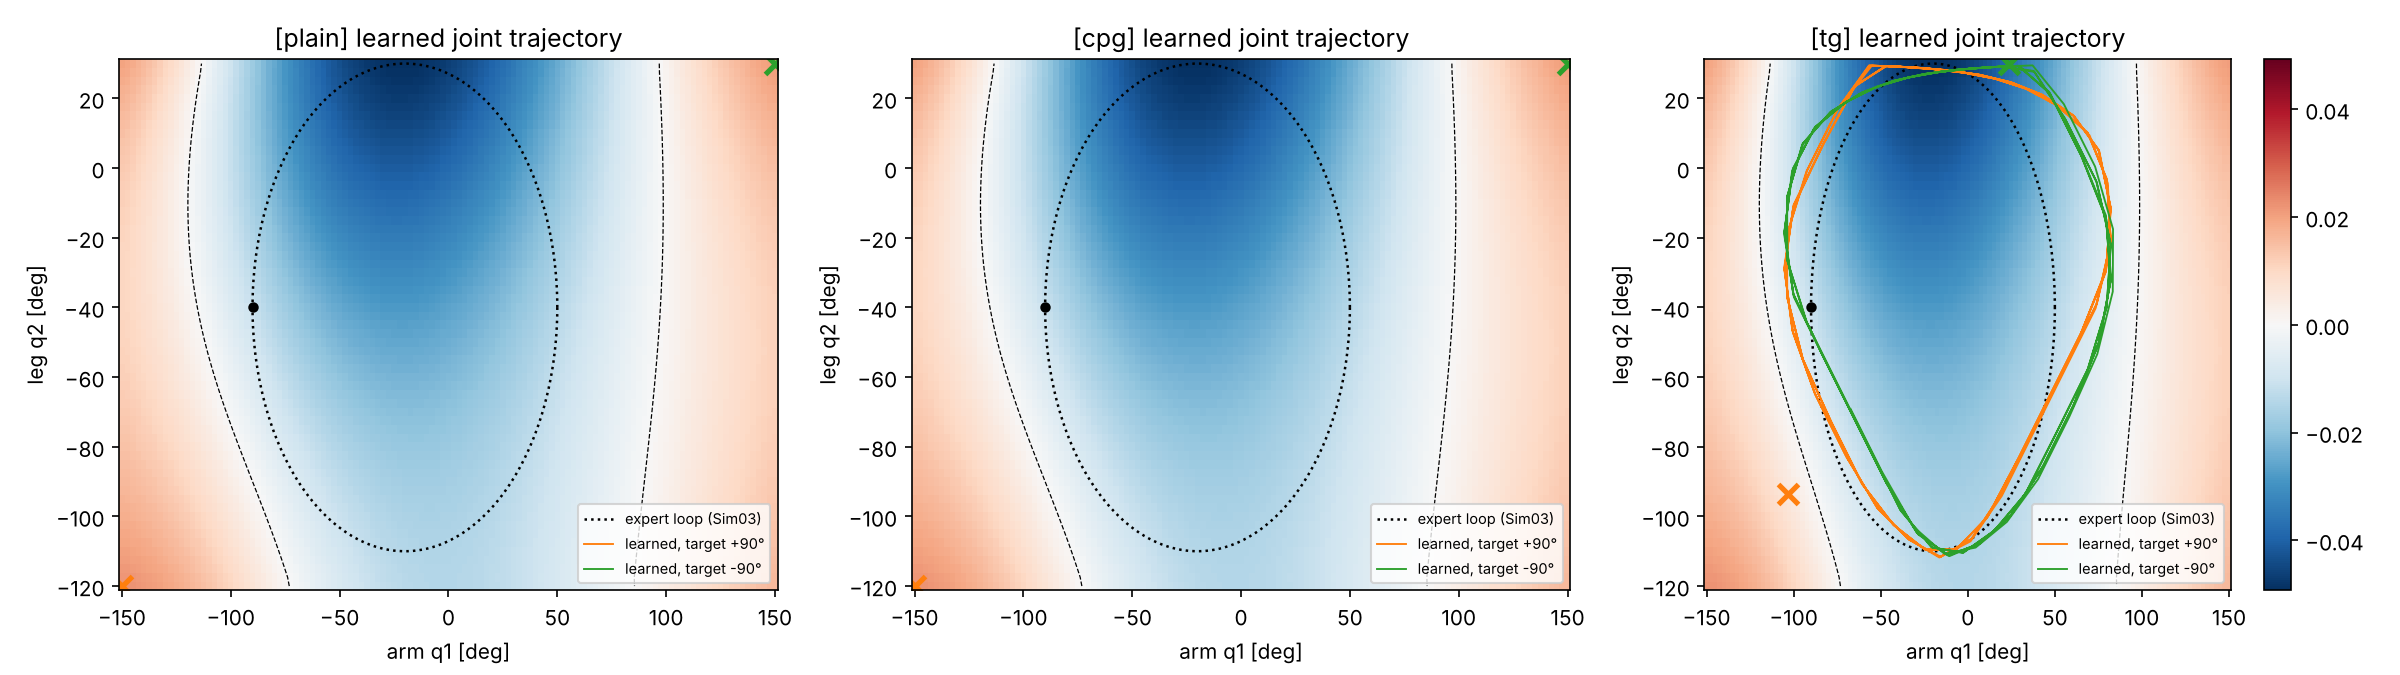
\includegraphics[width=0.86\textwidth]{figs/learn_top.png}
\caption{学習した関節の軌道（色は接続の曲率 $F$）。plain と cpg は手足を可動域の端まで振って止まる局所解（×印）に収束する。
振動子の構造を持つ tg は、曲率が負の領域をほぼ埋めるループを見つけた。点線は人手で設計した最適円ループ。}\label{fig:learn}
\end{figure*}

\textbf{結果}（表~\ref{tab:learn}、図~\ref{fig:learn}）：plain と cpg は、手足を可動域の端まで振って止まる局所解に収束した。
tg は数十イテレーションで解を見つけ、1 周 $+9.34^\circ$ のループを学習した。これは人手で設計した最適円（$+6.70^\circ$）を上回り、可動域内の理論上界（$+9.57^\circ$）の 98\% に達する。
回す向きも曲率の符号と整合し、最後に「揺れの少ない位相で止まる」ことまで覚えて、終端誤差は expert より 1 桁以上小さかった。

\textbf{なぜ構造なしでは失敗するのか}：1 回の動きの効果（可逆な首振り $-\bm\Gamma\cdot\Delta\bm q$）は振幅の 1 次だが、ループの正味の回転（曲率 × 囲んだ面積）は振幅の 2 次（$\propto A_1A_2$）である。
静止に近い方策から探索を始めると、ループを大きくする方向の勾配はほぼ 0 になり、1 次の効果である「端まで振る」が先に最適化される。
これはハイパーパラメータの問題ではなく、課題の物理構造に由来する。周期信号を観測に足すだけ（cpg）では足りず、「ループを描く」という\textbf{形}を方策の構造として与えることが成否を分けた。

同じ現象は地上でも現れた。MuJoCo \cite{todorov2012} を評価関数として直接使い、荷物運びの腰と肘の動きを Nelder--Mead 法で最適化したところ、
最初から短い動作時間で探すとどの係数でも転倒して評価が平らになり、探索が進まなかった。
時間を少しずつ短くする継続法で、荷物運びの時間は 65\% 短縮し、「反ってから前に傾く」という人が重い物を持つときの動き（腰の戦略）が再発見された。
\textbf{評価が平らになる領域を、物理の構造から予測し、避ける設計}が、安価なシミュレーションで事前に検討できる。

\section{課題 2：モデル誤差と、学習・最適制御の分担}

\textbf{設定}：18 m 級の機体で、スラスタと AMBAC を併用して 90° の旋回を 60 s で行う。
制御器は周回平均の「平均化モデル」しか知らず、評価には周回内の揺れを含む「位相モデル」を用いる（モデル誤差）。
さらにループ形状の効き（$\times0.7$〜$1.3$）、慣性（$\times0.9$〜$1.1$）、一定の外乱トルクをランダムに変えた 100 例で比べた。
学習方策は観測（平均姿勢の誤差、角運動量、残り時間、ループの位相）からスラスタのトルクとループの周波数を出す MLP で、同じランダムな条件で学習した（ドメインランダム化 \cite{peng2018}）。

\begin{table}[t]\centering\small
\caption{モデル誤差・外乱がある 100 例での比較}\label{tab:robust}
\setlength{\tabcolsep}{4pt}\begin{tabular}{lccc}\toprule
制御器 & 終端誤差 & 残留角速度 & 推進剤 \\
 & 平均（95\%） & [°/s] & [kg] \\\midrule
開ループ最適制御 & 30.5°（68.8°） & 0.90 & \textbf{1.97} \\
MPC & 14.6°（23.3°） & 0.030 & 5.41 \\
MPC＋揺れ補償 & 0.19°（0.69°） & 0.031 & 5.56 \\
学習方策 & \textbf{0.09°（0.10°）} & \textbf{0.002} & 4.92 \\\bottomrule
\end{tabular}
\vspace{1pt}\par\footnotesize 参考：公称モデルでのスラスタのみの最適値は 3.62 kg。
\end{table}

\textbf{結果}（表~\ref{tab:robust}）：線形計画で解いた開ループの最適制御は、推進剤は最小だが、終端誤差が 30° に達した。
平均化モデルの予測自体は正確（平均姿勢 89.6° 対予測 90.0°）で、誤差の原因は止まった位相での揺れだった。
人手で揺れの補償を加えた MPC は誤差 0.19° まで改善したが、学習方策は\textbf{観測に位相を入れただけで}同じことを自力で獲得し、誤差 0.09°、残留回転は MPC の 1/10 だった。
実行時の計算も行列積だけで済む（100 例で 0.1 s 対 LP の再計画で 15〜40 s）。

一方、学習方策の推進剤は、スラスタだけの最適値より多かった。
スラスタで角運動量を一度入れると、止めるときに同じ量の逆噴射が必ず要るため、\textbf{AMBAC が推進剤を節約できるのは「最初にどれだけ噴くか」を決める段階だけ}である。
報酬が終端でしか与えられない学習では、この最初の判断の価値を割り当てにくく（信用割り当ての問題）、学習方策は AMBAC で得をする余地を自ら消していた。

\textbf{示唆}：保存量（角運動量）の収支のように、最適性が明示的な構造で決まる部分は最適制御で計画し、
モデル誤差・外乱・速い揺れの補正は学習で担う、という分担（残差学習 \cite{johannink2019}）が自然である。
第 3 節と合わせると、\textbf{「形」（ループ）は方策の構造として与え、「保存量」は計画で扱う}という、物理の知識と学習の分担の指針が得られる。
安価なシミュレーションでも、両者の得意・不得意を同じ条件で切り分けられる。

\section{課題 3：校正値を実機の前に設計する}

本節は進行中の研究である。
物理エンジン MuJoCo（CPU のみ）上に、障害物のない試験環境と、段差・坂・低摩擦面・低重力などの評価環境を用意し、部品表から機体を組み立てて動かす。

\textbf{シミュレータ自体の照合}：まず、第 3・4 節で用いた Python の基準モデルと MuJoCo を同じ関節の動きで比べた。
腕 1 本の往復で $-16.0356^\circ$ 対 $-16.0356^\circ$、腕＋脚のループ 1 周で $+2.963^\circ$ 対 $+2.970^\circ$ と一致し、角運動量の保存は $10^{-6}$ 程度だった（この照合は積分法 RK4 による）。
ゲーム用の物理エンジンは安定化のための減衰などで角運動量が厳密には保存されないことがあり、1 周数度の幾何学的位相は埋もれうる。
\textbf{答えの分かっている試験に合格させること自体が、シミュレータの校正}になる。
将来の実機を 3 層目とし、基準モデル・シミュレーション場・実機の 3 層で照合する。

\begin{figure*}[t]\centering
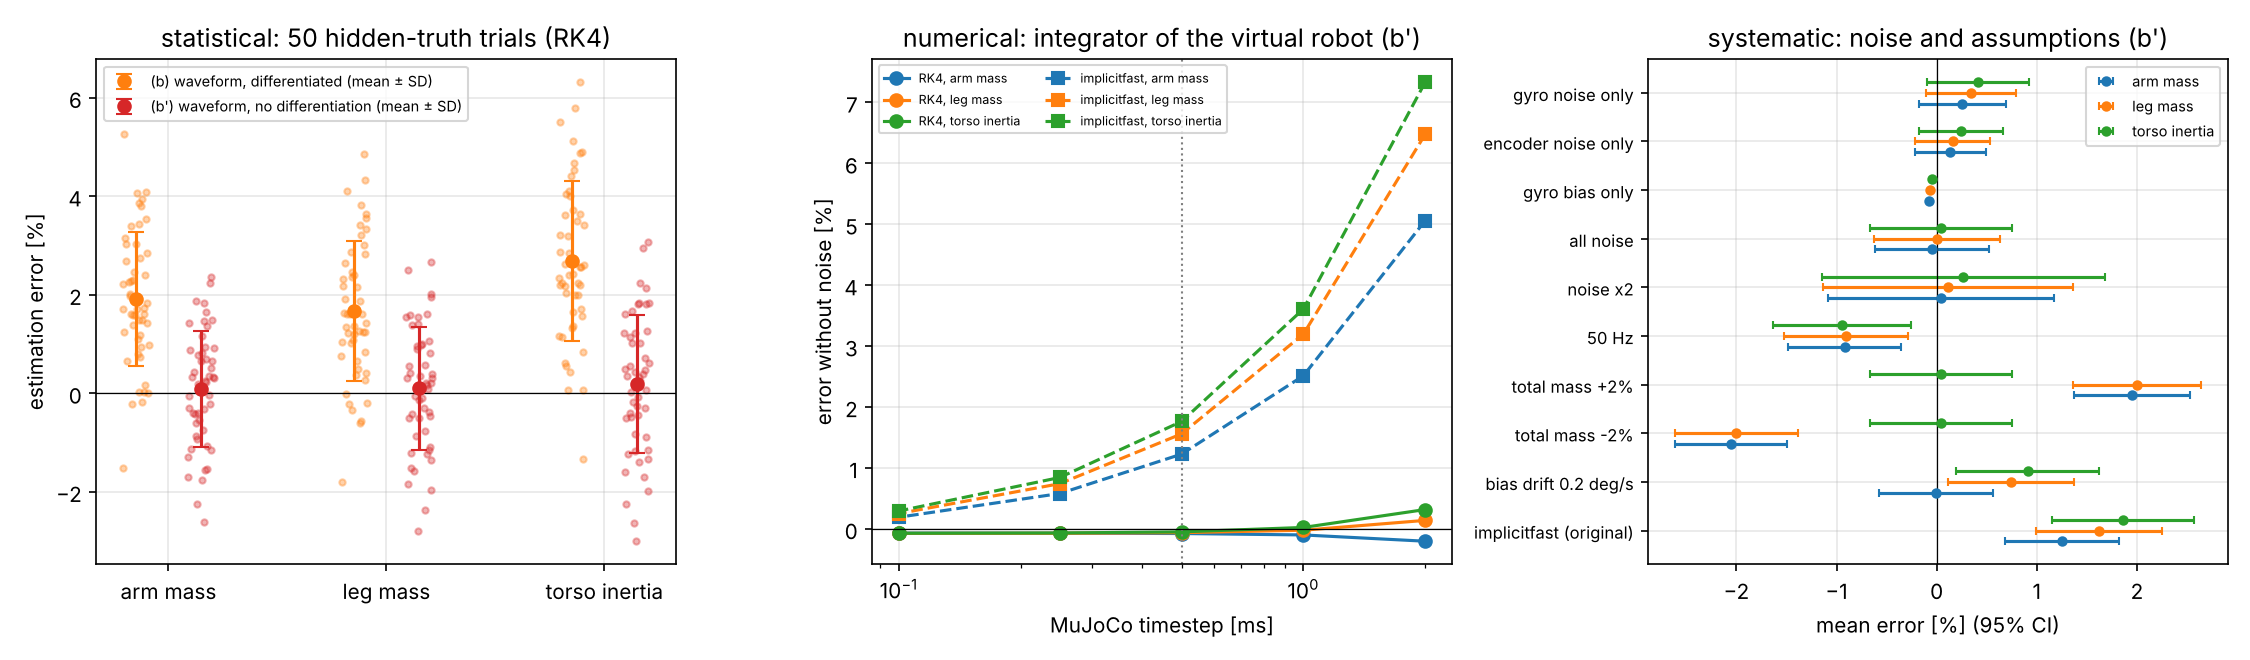
\includegraphics[width=0.84\textwidth]{figs/error_budget.png}
\caption{答えを隠した仮想の実機による校正の誤差評価。左：統計誤差（正解と雑音を変えた 50 回の試行、点は各試行、誤差棒は平均 $\pm$ 標準偏差）。
中：計算誤差（雑音なしの推定誤差と、仮想の実機の時間刻み・積分法。点線は既定の 0.5 ms）。
右：系統誤差（雑音の種類と推定側の仮定を 1 つずつ変えたときの平均の偏り、誤差棒は 20 通りの雑音による 95\% 信頼区間）。}\label{fig:calib}
\end{figure*}

\textbf{答えを隠した仮想の実機}：実機の代わりに、腕・脚の質量（$\pm15\%$）と胴体の慣性（$\pm10\%$）を乱数でずらした機体を作り、正解を推定する側に隠した（総質量 76 kg は既知とする）。
曲率マップの異なる場所に置いた 6 種類のループを 1 周ずつ回し、ジャイロ（雑音 0.2°/s、一定のバイアス最大 $\pm0.2$°/s）とエンコーダ（雑音 0.05°）を 100 Hz で模擬記録して、推定結果を正解と比べた。
推定法は、(a) 1 周ごとの正味の回転だけ、(b) 周回中の角速度の波形（関節角を微分して $\dot{\bm q}$ を求める）、
(b$'$) 式~(\ref{eq:ambac}) が時間を含まないことを利用し、0.1 s の区間ごとの回転量を $-\int\bm\Gamma\cdot d\bm q$ と比べる（微分なし）の 3 つである。いずれもジャイロのバイアスを同時に推定する。

\begin{table}[t]\centering\small
\caption{推定誤差（50 回の平均 $\pm$ 標準偏差 [\%]）。平均の 95\% 信頼区間の半幅は (b)(b$'$) で 0.3〜0.45\%。}\label{tab:calib}
\footnotesize\setlength{\tabcolsep}{2pt}
\begin{tabular}{lccc}\toprule
推定の方法 & 腕 & 脚 & 慣性 \\\midrule
(a) 正味の回転 & $-7\pm28$ & $+103\pm145$ & $+16\pm42$ \\
(b) 微分 & $+1.9\pm1.4$ & $+1.7\pm1.4$ & $+2.7\pm1.6$ \\
(b$'$) 微分なし & $\bm{+0.09\pm1.17}$ & $\bm{+0.10\pm1.25}$ & $\bm{+0.18\pm1.40}$ \\\bottomrule
\end{tabular}
\end{table}

\begin{table}[t]\centering\small
\caption{(b$'$) の誤差の内訳 [\%]（腕 / 脚 / 慣性）}\label{tab:budget}
\setlength{\tabcolsep}{3pt}
\begin{tabular}{p{0.52\linewidth}c}\toprule
誤差の種類 & 大きさ \\\midrule
\multicolumn{2}{l}{\textbf{統計誤差}} \\
\quad 1 試行の標準偏差 & 1.2 / 1.3 / 1.4 \\
\quad 50 回の平均の 95\% 信頼区間 & $\pm$0.33 / 0.35 / 0.39 \\
\multicolumn{2}{l}{\textbf{計算誤差}（雑音なし）} \\
\quad 時間刻み 0.5→0.1 ms（RK4） & 0.02 以下 \\
\quad 最適化の収束条件 & 0.001 以下 \\
\quad 推定式の離散化・モデル差 & $-0.07$ \\
\quad 積分法 implicitfast（0.5 ms） & \textbf{+1.2 / +1.6 / +1.8} \\
\multicolumn{2}{l}{\textbf{系統誤差}（20 通りの雑音の平均）} \\
\quad 雑音による偏り（全雑音） & $-0.05$ / 0.00 / +0.05 \\
\quad 総質量の仮定 $\pm2\%$ & $\pm2.0$ / $\pm2.0$ / 0.0 \\
\quad バイアスのドリフト 0.2°/s & 0.0 / +0.7 / +0.9 \\
\quad サンプリング 50 Hz & $-0.9$ / $-0.9$ / $-0.9$ \\\bottomrule
\end{tabular}
\end{table}

\textbf{結果}（図~\ref{fig:calib}、表~\ref{tab:calib}・\ref{tab:budget}）：
\textbf{統計誤差}：ループ 1 周の正味の回転だけ (a) では、脚の質量を推定できなかった。
波形を使う (b) と (b$'$) の 1 試行のばらつきは 1.2〜1.6\% で、主にジャイロの雑音による（ジャイロの雑音だけで 1.0\%）。
(b$'$) の 50 回の平均は 0.2\% 以下で、95\% 信頼区間が 0 を含み、偏りは統計的に有意でない。
\textbf{系統誤差}：(b) は +1.7〜2.7\% 偏り、信頼区間は 0 を含まない。偏りはエンコーダの雑音だけでも生じ、サンプリングを 200 Hz に上げると +3〜7\% に増え、雑音を 2 倍にしても増えた。
雑音の入った関節角を微分して推定式に入れると偏る errors-in-variables の典型であり、微分を避けた (b$'$) にはこの偏りがない。
推定側の仮定では、既知とした総質量の誤差が腕・脚の質量にそのまま 1:1 で移り、バイアスのドリフトとサンプリングの粗さが 1\% 弱の偏りを生んだ。

\textbf{計算誤差 --- シミュレータ自身が系統誤差の源になる}：
当初、仮想の実機は部品表から組み立てた MuJoCo のモデルを既定の積分法 implicitfast（1 次）で計算しており、(b$'$) は約 2\% の誤差を示していた。
雑音を除いても +1.2〜1.8\% の偏りが残り、偏りは時間刻みに比例した（2 ms で +5〜7\%、0.1 ms で +0.2〜0.3\%）。
原因は、1 次の積分法で角運動量 $L=0$ がわずかに保たれないことにある。式~(\ref{eq:ambac}) からのずれは姿勢の角速度の 0.02\% 程度にすぎないが、
推定はこのずれを、次に述べる推定しにくい方向（全体の大きさ）に沿って吸収するため、パラメータでは 2 桁大きい偏りになる。
積分法を RK4 にすると、0.5 ms でも雑音なしの誤差は 0.08\% 以下になった。
\textbf{答えを隠した仮想の実機で校正を設計するとき、仮想の実機自身の数値誤差が、推定しにくい方向で拡大されて系統誤差として現れる}。
これを見逃すと、推定法の限界や前処理の問題と取り違える（我々も当初は、偏りの原因を前処理だけに帰していた）。
仮想の実機の数値設定は、答えの分かっている保存則（ここでは $L=0$）で事前に検証しておく必要がある。

さらに、腕・脚の質量と胴体の慣性が\textbf{そろって同じ割合で増減する方向}が推定しにくい（特異値がほかの方向の約 1/60）ことが分かった。
式~(\ref{eq:ambac}) は質量・慣性の「比」しか含まないため、姿勢の波形だけでは全体の大きさが決まらない。
これはマニピュレータの同定で知られる「推定可能なパラメータの組み合わせ」\cite{gautier1990} と同じ構造で、
総質量の誤差が質量の推定に 1:1 で移ることも、この構造の表れである。\textbf{絶対値を決めるには、総質量の正確な計量か、関節トルクなどの力の情報が要る}。ただし力の情報を関節角の 2 回の微分と組み合わせると、上と同じ理由で偏る（元の条件の 5 回の試行で、誤差は 4〜5\% に悪化した）ため、速度・加速度を直接測るセンサーとの組み合わせが必要になる。

\textbf{拘束条件つきの当てはめによる誤差の自己評価}：
実機では正解が分からないため、校正値そのものに加えて「その値をどこまで信じてよいか」を、1 回の校正から示せる必要がある。
そこで、素粒子実験の kinematic fit \cite{avery1998} の考え方を校正に持ち込んだ。
関節角も誤差のある測定値として、その誤差の範囲で動かし、角運動量 $L=0$ を拘束条件として厳密に満たすように、真の関節角の列 $\bm Q$・パラメータ $\bm p$・ジャイロのバイアス $b$ をまとめて当てはめる。
{\small\begin{equation}
\chi^2=\sum_i\frac{\|\bm Q_i-\bm q_{m,i}\|^2}{\sigma_q^2}+\sum_i\frac{\bigl(\omega_{m,i}-b+\bm\Gamma(\bm Q_i;\bm p)\cdot\dot{\bm Q}_i\bigr)^2}{\sigma_\omega^2}
\label{eq:kinfit}
\end{equation}}
$\dot{\bm Q}_i$ は当てはめた $\bm Q$ の中心差分で、雑音の入った測定値を微分しないため、(b) のような偏りは生じない。
未知数は約 5200 個だが、ヤコビアンが疎なので、CPU で 1 回 50 s 程度で解ける。
得られた共分散から、推定ごとの誤差 $\sigma$ と、当てはまりの良さ $\chi^2$ が得られる。

\begin{figure*}[t]\centering
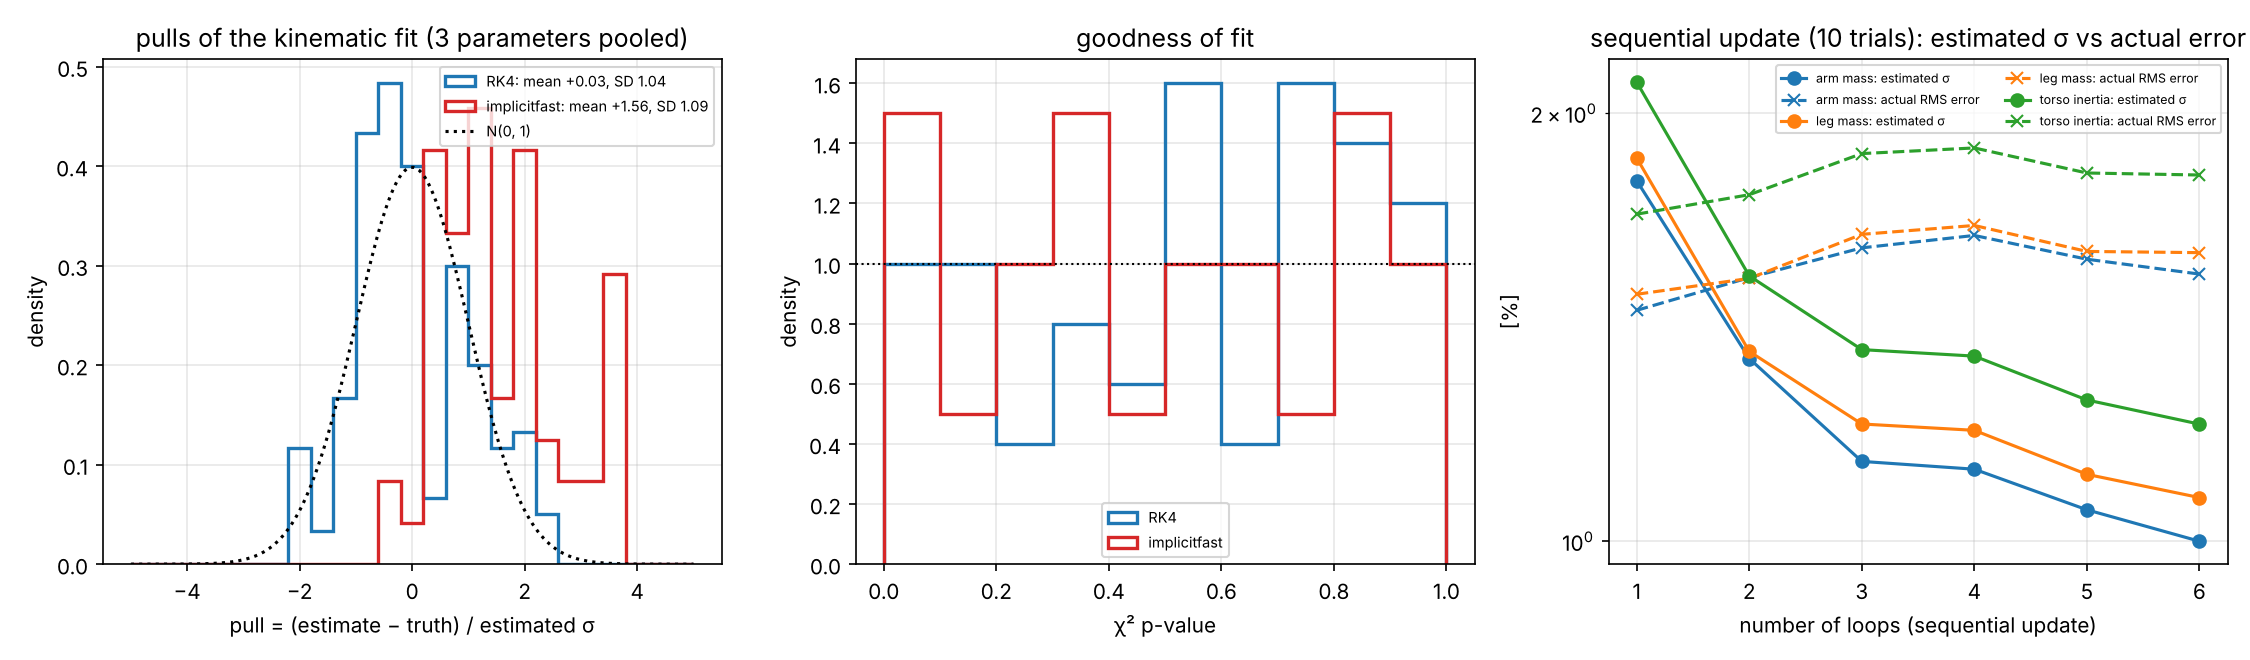
\includegraphics[width=0.84\textwidth]{figs/kinfit.png}
\caption{拘束条件つきの当てはめ（式~(\ref{eq:kinfit})）の自己評価。左：pull $=(\text{推定}-\text{正解})/\sigma$ の分布（3 つのパラメータをまとめた）。RK4 の仮想の実機（50 回）では $N(0,1)$ に一致し、積分法の系統誤差を含む implicitfast（20 回）では $+1.6\sigma$ ずれる。
中：$\chi^2$ の p 値。どちらも一様で、系統誤差は $\chi^2$ に現れない。右：ループを 1 本ずつ加える逐次更新での、推定した $\sigma$（実線）と実際の誤差の二乗平均（破線、10 回）。}\label{fig:kinfit}
\end{figure*}

結果を図~\ref{fig:kinfit} に示す。RK4 の仮想の実機での 50 回の試行で、推定は偏らず（平均 0.04\% 以下）、ばらつきは 1.1〜1.3\% で (b$'$) より約 3 割小さかった。
\textbf{推定ごとの誤差 $\sigma$ は正しく見積もられ}、pull の平均は 0.01〜0.05、標準偏差は 1.04〜1.05、$|\text{pull}|<1$ の割合は 66〜68\% で、$\chi^2/\text{ndf}=0.997\pm0.032$ だった。
ループを 1 本ずつ加え、前の推定値と共分散を事前情報として当てはめ直す逐次更新（カルマンフィルタと同じ形で、素粒子実験の飛跡の当てはめ \cite{fruhwirth1987} でも用いられる）では、
$\sigma$ はループを加えるごとに 1.8\% から 1.0\% へ縮み、最終値は一括の当てはめと 0.23\% 以内で一致した。
一方、積分法の系統誤差を含む仮想の実機では、pull は $+1.4$〜$1.6\sigma$ ずれたが、\textbf{$\chi^2$ の p 値は一様のままで、当てはまりの良さからは検出できなかった}。
3 つのパラメータの推定の相関係数が 0.99 以上あり、ずれが推定しにくい方向に吸収されるためである。
拘束条件つきの当てはめは誤差の自己評価を与えるが、推定しにくい方向の系統誤差は、正解の分かっている照合など独立な検証と組み合わせて評価し続ける必要がある。

\textbf{どの校正値が効くか}：組み立てた機体を試験した結果、次の量が性能を大きく左右した。
(i) 重力だけが違うステージでは、荷物運びの安全な最短時間がフルード則（$\propto\sqrt{\text{大きさ}/g}$）で 1\% の精度で移せたが、氷では外れ（予測 1.35 s 対 2.22 s）、制約が転倒から滑りに変わる。摩擦は重力のスケーリングとは別の校正値になる。
(ii) 接地の荷重分布を一様と仮定すると、履帯の旋回の速さを 3 割ずれて見積もる。
(iii) 地上で腕を振ると、足元の摩擦が車体を回し始めるトルク（この機体で約 260 N·m）までは反作用を吸収する。車体を乱すのは主に腕を\textbf{止めるとき}で、位置サーボの遅れ（最大 17°）が急ブレーキを生み、この境目を超えさせていた。
(iv) 宇宙の試験場でも、基準値とのわずかなずれはサーボの追従遅れによるもので、\textbf{アクチュエータの特性がそのまま姿勢の誤差になる}。
これらは、\textbf{モデルに含めた誤差源の中で}、実機で何を先に測るべきかの候補を与える。

\section{考察}

\textbf{安価なシミュレーションに答えられること}：
本稿の 3 つの課題で、シミュレーションは「実機の挙動の予測」ではなく、
\textbf{(1) 学習に与えるべき構造、(2) 学習と制御の分担、(3) 校正の試験動作と測るべき量}を決めるために使われた。
いずれも、答えの分かっている試験台があるから判断できた。
大規模な GPU シミュレーションとドメインランダム化が「誤差の範囲を広く覆う」方向だとすると、本稿の方向は「どこに誤差があり、何を測ればよいか」を絞る方向であり、両者は補完的になりうる。ただし、これは本稿の事例に基づく仮説であり、両者を同じ課題で比べた検証は行っていない。

\textbf{一般化の射程}：第 3 節の失敗の原因（正味の効果が入力の 2 次、すなわちリー括弧から生じる）は AMBAC に固有ではなく、
車両の縦列駐車に代表される非ホロノミック系、自由浮遊宇宙ロボット \cite{nakamura1991}、ヘビ型・遊泳型の移動など、形状の周期運動で全体を動かす系に共通する。
これらの系では正弦波入力による操舵 \cite{murray1993} が古典的な解法であり、振動子の構造が有効だったことと整合する。
したがって「構造なしの探索は 2 次の効果の前で停滞し、周期運動の構造で解消する」という仮説は、この系の族に対して検証可能な形で立てられる。
一方、接触の細部、アクチュエータの非線形、柔軟体のように、誤差の主因がモデルの外にある課題には、本稿の枠組みは直接は届かない。

\textbf{答えられないこと}：PC の上だけでは sim-to-real ギャップそのものは確かめられない。
仮想の実機で絞り込めるのは、モデルに含めたパラメータについて、推定しやすい方向・しにくい方向と、前処理などの手順上の落とし穴までである。
モデルに入れていない現象（接触の細部、モーターの非線形、部品のたわみ）は再現されず、\textbf{実機で初めて効いてくる未知の誤差源の優先順位は決められない}。
アクチュエータの数値は仮定の部品の値に基づく。

\textbf{学習手法の限定}：本稿の学習はすべて ES による。構造を与える効果が ES に特有のものか、PPO や SAC などの勾配に基づく強化学習を含むモデルフリー学習一般に成り立つかは、本稿の結果からは判断できない。
勾配に基づく手法では探索の初期の方策のばらつきが異なるため、2 次の効果による停滞の程度も変わりうる。同じ試験台で複数の学習法を比べることが、本稿の主張を強めるための最優先の課題である。

\textbf{今後の目標}：
(1) 同じ試験台での PPO・SAC との比較と、他の非ホロノミック系（正弦波操舵の古典例など）での構造仮説の検証、
(2) 計画を最適制御、実行時の補正を学習方策が担うハイブリッド制御の実装、
(3) 安価なサーボのアーム 1 台による 3 層目（実機）の照合と、仮想の実機で設計した校正手順の実機での確認、
(4) 拘束条件つきの当てはめに、アクチュエータ・摩擦の校正値と実機のデータを逐次加え、誤差を評価し続ける校正の枠組みへの拡張、(5) 校正データを公開し、機械学習による推定と物理モデルによる推定を同じデータで比べること、を進める。

\section{まとめ}

実機も高精細なシミュレータも持たない条件で、CPU だけで動く安価なシミュレーションがフィジカル AI の課題にどこまで答えられるかを、AMBAC を試験台に検討した。
構造のない学習の失敗を物理の 2 次の効果として説明し、振動子の構造を与えた学習が理論上界の 98\% に達すること、
モデル誤差の下では学習が頑健だが保存量の計画は最適制御が担うべきこと、
答えを隠した仮想の実機で、校正の誤差を統計・計算・系統に分けて評価し、推定の手順と測るべき量を実機の前に絞り込めること、拘束条件つきの当てはめで推定ごとの誤差を正しく見積もれること、ただし仮想の実機自身の数値誤差が系統誤差の源になり、それは当てはまりの良さに現れないことを示した。いずれも ES を用いた単一の系での事例であり、一般化は今後の検証による。
安価なシミュレーションは実機の代わりではなく、\textbf{実機に何を持ち込むべきかを決める道具}として、計算資源の限られた研究者にも開かれている。

\begin{thebibliography}{99}\footnotesize\setlength{\itemsep}{0pt}
\bibitem{tobin2017} J.~Tobin et al., ``Domain randomization for transferring deep neural networks from simulation to the real world,'' \textit{IROS}, 2017.
\bibitem{peng2018} X.~B.~Peng, M.~Andrychowicz, W.~Zaremba, P.~Abbeel, ``Sim-to-real transfer of robotic control with dynamics randomization,'' \textit{ICRA}, 2018.
\bibitem{hwangbo2019} J.~Hwangbo et al., ``Learning agile and dynamic motor skills for legged robots,'' \textit{Science Robotics}, 4(26), 2019.
\bibitem{ijspeert2008} A.~J.~Ijspeert, ``Central pattern generators for locomotion control in animals and robots: a review,'' \textit{Neural Networks}, 21(4), 642--653, 2008.
\bibitem{iscen2018} A.~Iscen et al., ``Policies modulating trajectory generators,'' \textit{CoRL}, PMLR 87, 916--926, 2018.
\bibitem{atkeson1986} C.~G.~Atkeson, C.~H.~An, J.~M.~Hollerbach, ``Estimation of inertial parameters of manipulator loads and links,'' \textit{IJRR}, 5(3), 101--119, 1986.
\bibitem{gautier1990} M.~Gautier, W.~Khalil, ``Direct calculation of minimum set of inertial parameters of serial robots,'' \textit{IEEE Trans. Robotics and Automation}, 6(3), 368--373, 1990.
\bibitem{makoviychuk2021} V.~Makoviychuk et al., ``Isaac Gym: High performance GPU-based physics simulation for robot learning,'' \textit{NeurIPS Datasets and Benchmarks}, 2021.
\bibitem{kane1970} T.~R.~Kane, M.~P.~Scher, ``Human self-rotation by means of limb movements,'' \textit{J. Biomechanics}, 3(1), 39--49, 1970.
\bibitem{kane1969} T.~R.~Kane, M.~P.~Scher, ``A dynamical explanation of the falling cat phenomenon,'' \textit{Int. J. Solids and Structures}, 5(7), 663--670, 1969.
\bibitem{montgomery1993} R.~Montgomery, ``Gauge theory of the falling cat,'' in \textit{Dynamics and Control of Mechanical Systems}, Fields Inst. Commun. 1, AMS, 1993.
\bibitem{marsden1992} J.~E.~Marsden, \textit{Lectures on Mechanics}, Cambridge University Press, 1992.
\bibitem{brockett1983} R.~W.~Brockett, ``Asymptotic stability and feedback stabilization,'' in \textit{Differential Geometric Control Theory}, Birkhäuser, 181--191, 1983.
\bibitem{salimans2017} T.~Salimans et al., ``Evolution strategies as a scalable alternative to reinforcement learning,'' arXiv:1703.03864, 2017.
\bibitem{todorov2012} E.~Todorov, T.~Erez, Y.~Tassa, ``MuJoCo: A physics engine for model-based control,'' \textit{IROS}, 2012.
\bibitem{nakamura1991} Y.~Nakamura, R.~Mukherjee, ``Nonholonomic path planning of space robots via a bidirectional approach,'' \textit{IEEE Trans. Robotics and Automation}, 7(4), 500--514, 1991.
\bibitem{murray1993} R.~M.~Murray, S.~S.~Sastry, ``Nonholonomic motion planning: steering using sinusoids,'' \textit{IEEE Trans. Automatic Control}, 38(5), 700--716, 1993.
\bibitem{avery1998} P.~Avery, ``Applied fitting theory VI: Formulas for kinematic fitting,'' CLEO Note CBX 98-37, 1998.
\bibitem{fruhwirth1987} R.~Frühwirth, ``Application of Kalman filtering to track and vertex fitting,'' \textit{Nucl. Instrum. Methods A}, 262, 444--450, 1987.
\bibitem{johannink2019} T.~Johannink et al., ``Residual reinforcement learning for robot control,'' \textit{ICRA}, 2019.
\end{thebibliography}

\end{document}
